\documentclass[../../main.tex]{subfiles}

\begin{document}

\setchapterpreamble[u]{\margintoc}

\chapter{树}

树是一个十分重要的数据结构,尤其以二叉树为例。本章主要记录如何解决一些树相关的问题。

\section{二叉树的遍历}

二叉树的遍历是一个十分重要的问题,我们可以使用递归的方式来解决这个问题,但是递归的方式十分的简单,本节
主要介绍使用非递归的方式实现二叉树的遍历。

\subsection{\href{https://leetcode.cn/problems/binary-tree-preorder-traversal/}
{二叉树的前序遍历}}

我们举一个简单的例子,来说明如何使用迭代的方式实现二叉树的前序遍历。如下图所示,我们首先需要访问
根节点5,然后需要访问其左节点。这就来到了问题的关键地方,我们必须保存节点5,以便在遍历完其左孩子,
能够访问其右孩子。对于每一个节点,我们都这样操作\sidenote{在此处,我忽略了细节的操作,实际上我认为
我们掌握这个思维方式才是最重要的,这样我们就能写出循环了,因为每一个节点都是这样的。}。

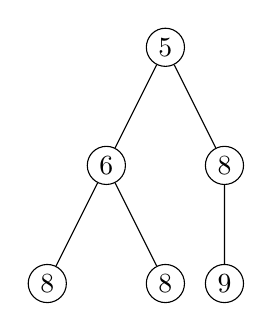
\begin{tikzpicture}[every node/.style={draw, circle, inner sep=2pt}]
  \node {5}
    child {node {6}
      child {node {8}}
      child {node {8}}
    }
    child {node {8}
      child {node {9}}
    };
\end{tikzpicture}

这样,我们就可以写出如下的代码:

\lstinputlisting[language=C++]{code/binary-tree-preorder-traversal.cpp}

\subsection{\href{https://leetcode.cn/problems/binary-tree-inorder-traversal/}
{二叉树的中序遍历}}

当我们写出了二叉树的前序遍历,我们就能写出二叉树的中序遍历了。我们只需要将前序遍历的代码稍作修改即可。
我们需要将节点保存在栈中,当我们访问完左孩子后,再访问中间节点。

\lstinputlisting[language=C++]{code/binary-tree-inorder-traversal.cpp}

\subsection{\href{https://leetcode.cn/problems/binary-tree-postorder-traversal/}
{二叉树的后序遍历}}

二叉树的后序遍历是使用迭代方法最难写的一个算法。因为我们必须在最后访问根节点,但是我们并不知道何时
这个节点的右子树已经遍历完成了,所以我们可以使用一个变量\texttt{pre}来保存上一次访问的节点,如果
当前节点的右子树已经遍历完成了,那么我们就可以访问当前节点了。即\texttt{ptr->right == pre}。
通过这个小技巧,我们就可以得出二叉树的后序遍历的非递归算法了。

\begin{kaobox}[title=二叉树统一迭代遍历方法]
  通过上述的三个代码,我们已经总结出了二叉树统一迭代遍历的方法。Amazing。
\end{kaobox}

\lstinputlisting[language=C++]{code/binary-tree-postorder-traversal.cpp}

\subsection{\href{https://leetcode-cn.com/problems/binary-tree-level-order-traversal/}
{二叉树的层序遍历}}

二叉树的层序遍历是典型的广度优先搜索算法,通过一个队列保存每层的节点即可,直到队列为空。

\lstinputlisting[language=C++]{code/binary-tree-level-order-traversal.cpp}

当解决了这个问题,我们可以解决如下的问题,其本质都是同一个思路:

\begin{itemize}
  \item \href{https://leetcode-cn.com/problems/binary-tree-zigzag-level-order-traversal/}
  {二叉树的锯齿形层序遍历}
  \item \href{https://leetcode.cn/problems/binary-tree-level-order-traversal-ii}
  {二叉树的层序遍历 II}
  \item \href{https://leetcode.cn/problems/average-of-levels-in-binary-tree}
  {二叉树的层平均值}
  \item \href{https://leetcode.cn/problems/n-ary-tree-level-order-traversal}
  {N叉树的层序遍历}
\end{itemize}

\section{二叉树的构建}

\subsection{\href{https://leetcode-cn.com/problems/construct-binary-tree-from-preorder-and-inorder-traversal/}
{从前序与中序遍历序列构造二叉树}}

要解决这个问题,我们首先需要思考前序遍历和中序遍历的特点。前序遍历的第一个节点一定是根节点,而中序遍历
的根节点左边的节点都是左子树的节点,右边的节点都是右子树的节点。因此,我们可以通过前序遍历的第一个节点
来确定根节点,然后在中序遍历中找到根节点的位置,然后递归地处理左子树和右子树。

然而,最关键的问题在于,我们应该先处理左子树还是右子树,这个问题的答案是,我们应该先处理左子树。因为
我们在前序遍历中,先访问的是根节点,然后是左子树,最后是右子树。因此,我们应该先处理左子树,然后再处理
右子树。为了快速地找到根节点在中序遍历中的位置,我们可以使用一个哈希表来存储中序遍历中每个节点的位置。

\lstinputlisting[language=C++]
{code/construct-binary-tree-from-preorder-and-inorder-traversal.cpp}

\subsection{\href{https://leetcode-cn.com/problems/construct-binary-tree-from-inorder-and-postorder-traversal/}
{从中序与后序遍历序列构造二叉树}}

这个问题和上一个问题的思路是一样的,只不过我们需要先处理右子树,然后再处理左子树。

\lstinputlisting[language=C++]{code/construct-binary-tree-from-inorder-and-postorder-traversal.cpp}

\subsection{\href{https://leetcode-cn.com/problems/construct-binary-tree-from-preorder-and-postorder-traversal/}
{根据前序和后序遍历构造二叉树}}

实际上前序遍历和后序遍历并不能唯一确定一棵二叉树,因为我们无法确定左子树和右子树的边界。但是,这个问题只需要
我们还原出任意一个符合条件的二叉树即可。

我们可以采取一个十分简单的思路。取当前节点的前序遍历的下一个节点作为其左子树的根节点,然后在后序遍历中确定该节点
的前一个节点作为其右子树的根节点。这样,我们就可以递归地构建出一棵二叉树了。但是这样我们还需要做一个工作,就是需要
记录这个节点是否已经被使用过了,如果使用过了,我们就不能再使用了。这个思路实际上并不能算上很优雅,但是这个解法
很直观且简单\sidenote{实际上,这个题确实是有更加优雅的做法。既然我们能够确定出当前节点的左子树的根节点以及其右子树
的根节点,那么我们就能够用长度的方式代替我们使用的\texttt{visited}变量,但我个人认为我这个思路是容易理解的。}。

\lstinputlisting[language=C++]{code/construct-binary-tree-from-preorder-and-postorder-traversal.cpp}

\section{二叉树的深度}

\subsection{\href{https://leetcode.cn/problems/maximum-depth-of-binary-tree/}{二叉树的最大深度}}

这个题我们只需要简单地使用递归进行处理即可,对于空节点,我们返回0,对于非空节点,我们返回左右子树的最大深度加1。
显然,利用二叉树的前序遍历我们就可以简单地得出如下的代码:

\lstinputlisting[language=C++]{code/maximum-depth-of-binary-tree.cpp}

\subsection{\href{https://leetcode-cn.com/problems/minimum-depth-of-binary-tree/}{二叉树的最小深度}}

似乎我们可以直接调用上一题的代码,把 。然而这样是不行的。因为如果我们的二叉树只有左子树或者只有右子树,那么我们的代码
会返回0,但是实际上这个二叉树的最小深度是3。如下图所示:

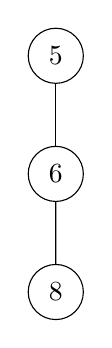
\begin{tikzpicture}[every node/.style={circle,draw,minimum size=7mm}]
  \node (5) {5}
    child {node (6) {6}
      child {node (8) {8}}};
\end{tikzpicture}

因此,当有某个节点其左子树或者右子树为空时,我们会得到其深度为0。当遇到了这样的情况,我们应该返回左子树
和右子树的最大的深度加1。当不会出现这样的情况时,我们就可以返回左子树和右子树的最小深度加1了。于是,我们
就可以得出如下的代码:

\lstinputlisting[language=C++]{code/minimum-depth-of-binary-tree.cpp}

\section{路径总和系列}

\subsection{\href{https://leetcode.cn/problems/path-sum/}{路径总和}}

这个题目是一个典型的深度优先搜索的题目。我们只需要递归地处理左子树和右子树即可。当我们遇到了叶子节点时,我们
判断当前的路径和是否等于目标值即可。

\lstinputlisting[language=C++]{code/path-sum.cpp}

\subsection{\href{https://leetcode-cn.com/problems/path-sum-ii/}{路径总和 II}}

这个题需要输出所有的路径,简单回溯即可。

\lstinputlisting[language=C++]{code/path-sum-ii.cpp}

\subsection{\href{https://leetcode-cn.com/problems/path-sum-iii/}{路径总和 III}}

首先,我们思考这个问题的暴力解法。我们可以枚举所有的节点,然后以这个节点为根节点,计算所有的路径和。
这样的时间复杂度会相当高。而且我们会有很多重复的计算。我们需要转化这个思路,我们首先假设这个路径
是一个数组。我们需要求和为$target$的子数组\sidenote{
实际上,我们此时已经把问题转化为了\href{https://leetcode.cn/problems/subarray-sum-equals-k/}{和为K的子数组}
}。对于数组$[a_{1}, a_{2}, \dots, a_{n}]$,我们希望找到$a_{i} + \dots + a_{j}$使得其和等于
$target$。然而,我们完全能转化这个问题。我们将其转化为

$$
a_{1} + a_{2} + \dots +a_{j} - (a_{1} + a_{2} + \dots + a_{i - 1}) = target
$$

对于上述上述公式,我们可以看出前面为当前的数组和,前者为前缀和。这样我们就将这个问题巧妙地转化为了
前缀和问题。我们可以使用一个哈希表来记录当前的前缀和出现的次数。然后使用$sum - target$去得到
当前前缀和的个数即可。

\lstinputlisting[language=C++]{code/path-sum-iii.cpp}

\subsection{\href{https://leetcode.cn/problems/binary-tree-maximum-path-sum/}
{二叉树中的最大路径和}}

这个题看似很难处理,实际上特别简单。对于一个节点,其最大路径和可能有四种情况:

\begin{itemize}
  \item 该节点的值
  \item 该节点的值加上左子树的最大路径和
  \item 该节点的值加上右子树的最大路径和
  \item 该节点的值加上左子树的最大路径和加上右子树的最大路径和
\end{itemize}

当需要往上传递路径的时候,我们最多选择一条路径,因此我们只需要比较前三种情况即可。所以我们先写出
网上传递的路径的最大值,再处理当前的最大路径和从而减少计算。

\lstinputlisting[language=C++]{code/binary-tree-maximum-path-sum.cpp}

\section{二叉搜索树的基本操作}

\subsection{\href{https://leetcode-cn.com/problems/search-in-a-binary-search-tree/}
{二叉搜索树中的搜索}}

本质上我们仍采用二分查找,只是我们基于二叉树做二分查找。

\lstinputlisting[language=C++]{code/search-in-a-binary-search-tree.cpp}

\subsection{\href{https://leetcode-cn.com/problems/insert-into-a-binary-search-tree/}
{二叉搜索树中的插入操作}}

如果不考虑平衡,二叉搜索树的插入是十分简单的,我们只需要找到插入的位置即可。我们需要两个指针,一个记录
当前节点,一个记录当前节点的父节点。当我们找到了插入的位置,我们就可以插入了。特别注意,父节点可能为
空,这样我们需要创建一个新的节点作为根节点。

\lstinputlisting[language=C++]{code/insert-into-a-binary-search-tree.cpp}

\subsection{\href{https://leetcode-cn.com/problems/delete-node-in-a-bst/}
{删除二叉搜索树中的节点}}

这个题目仍然是二叉搜索树的基本操作。然而虽说基本,但是需要分情况进行讨论\sidenote{
我直接使用了结论,然而你最好通过画图得出这个结论,没必要死记硬背。
}:

\begin{itemize}
  \item 如果删除的节点只有一个孩子,那么我们只需要将其孩子节点替换到当前节点即可。
  \item 如果删除的节点$delete$有两个孩子。我们需要做很多复杂的处理,我们需要找到比当前节点大的
  第一个节点$sucessor$。如果$sucessor$正好是$delete$的右孩子。我们只需要将$delete$替换为
  $successor$即可。如果不是。我们仍然将$delete$替换为$successor$即可。但是我们需要把
  $successor$的右孩子移动到$sucessor$的父节点的左孩子上。
\end{itemize}

\lstinputlisting[language=C++]{code/delete-node-in-a-bst.cpp}

\section{二叉搜索树的应用}

\subsection{\href{https://leetcode.cn/problems/convert-sorted-list-to-binary-search-tree/}
{有序链表转换二叉搜索树}}

把一个有序链表转化为二叉搜索树的过程是相当简单的,我们每次都取链表的中间节点作为根节点,然后递归地处理左子树和右子树
即可。

\lstinputlisting[language=C++]{code/convert-sorted-list-to-binary-search-tree.cpp}

\begin{kaobox}[title=类似题目]
  \begin{itemize}
    \item \href{https://leetcode.cn/problems/convert-sorted-array-to-binary-search-tree/}{将有序数组转换为二叉搜索树}
  \end{itemize}
\end{kaobox}

\subsection{\href{https://leetcode.cn/problems/convert-sorted-list-to-binary-search-tree/}
{验证二叉搜索树}}

对于这个题,我们可以直接使用迭代的方式进行处理。然而,我觉得用递归的方式更适合一些,显然我们要验证一个树是不是二叉
搜索树,我们需要去判断其值是不是严格递增的。我们可以使用一个变量来保存上一个节点的值,然后在递归的过程中进行判断。
这个变量必然需要是引用,因为其会在递归的下层被修改。

\lstinputlisting[language=C++]{code/validate-binary-search-tree.cpp}

\subsection{\href{https://leetcode.cn/problems/recover-binary-search-tree/}{恢复二叉搜索树}}

由于正好只有两个数被交换了,所以我们只要举例子就能就解决这个问题。例如$17345628$。显然我们需要找到$7$和$2$。
但是我们需要处理一个临界情况,就是$13245$,我们需要找到$3$和$2$。也就是每次我们寻找到上一个节点的值大于当前
节点的值,我们就需要记录下第二个节点。当第一个节点为空时,我们才记录第一个节点。

首先拿$17345628$为例,我们发现$7 > 3$,因此我们记录节点一,然后记录节点2。然后我们发现$6 > 2$。由于第一个
节点已经记录,我们只需要更新第2个节点。对于$13245$,我们只能发现$3 > 2$,同时记录了节点1和节点2。这样我们就
可以考虑到这个边界条件,进而我们可以写出如下的代码。

\lstinputlisting[language=C++]{code/recover-binary-search-tree.cpp}

\end{document}
